%%% Angepasste Version der unitext Vorlage von Dr. Werner Struckmann (https://www.tu-braunschweig.de/ips/staff/struckmann/unitext)
%%% für wissenschaftliche Arbeiten am Institut für Wirtschaftsinformatik, Abteilung Decision Support

%%% Die Klasse unitext besitzt die Optionen
%%% bachelorarbeit, projektarbeit, masterarbeit, studienarbeit, diplomarbeit,
%%% bericht und script für die verschiedenen Dokumenttypen. 
%%% Bei Bedarf k?nnen weitere aufgenommen werden. Aus jeder der beiden Gruppen ist
%%% genau eine Option zu wählen. Außerdem können der Stil des Literaturverzeich-
%%% nisses (alpha, abbrv, unsrt, plain, apalike) und die Sprache (german, english) als
%%% weitere Optionen angegeben werden. Die Angabe einer Sprache ist obligato-
%%% risch. Eine der Optionen dvi, ps oder pdf ist abhängig vom gewählten Ausgabe-
%%% format anzugeben. Dokumentspezifische Einstellungen werden in unitext.cfg
%%% vorgenommen. Der Text ist doppelseitig auszudrucken.
%%% Weitere Optionen: Beispiele für Titelseite: titelseite, cd

% pdf durch Ausgabeformat ersetzen: dvi, ps  oder pdf.

\documentclass[ds,english,bachelorarbeit,pdf,cd,apacite]{unitext} 

%\documentclass[ds,english,seminar,pdf,cd,apacite]{unitext}                % Default

        % Beispiel 1
% \documentclass[ds,german,masterarbeit,pdf,cd,apacite]{unitext}         % Beispiel 2

\usepackage{amsmath}
\DeclareMathOperator*{\argmin}{arg\,min}
\usepackage{graphicx}
\usepackage{subfigure}
\usepackage{enumitem}
\setlist[description]{leftmargin=\parindent,labelindent=\parindent}
\usepackage{hyperref}
\usepackage{natbib}
\usepackage{setspace}
\usepackage[section]{placeins}

\onehalfspacing
\overfullrule=0pt
%%% title, author und date m?ssen angegeben werden,
%%% dozent, betreuer und keywords sind optional.
\title{Comparison of Supervised Learning Methods for Arrival Time Estimation in Meal Delivery}
\author{Emre Gezer}
\matrikelnummer{4901507}
\studiengang{Wirtschaftsinformatik}

\dozent{Jun.-Prof. Dr. Marlin Ulmer}
\betreuer{M. Sc. Florentin D. Hildebrandt}

\date{10.02.2021} %%% Abgabedatum

\keywords{Wirtschaftsinformatik, Decision Support}


\makeglossary           %%% optional
\makeindex              %%% optional


\begin{document}

%%% Titelteil
\titelblatt             %%% obligatorisch
\tableofcontents        %%% obligatorisch
\erklaerung             %%% obligatorisch fuer Abschlussarbeiten
%listoftables           %%% optional
\listoffigures          %%% optional
%\abkuerzung             %%% optional, in der Datei abkuerzung.tex


%%% ------------- Der Textteil -------------
\starttext              

\chapter{Introduction}
%%% Motiviere Problem
Nobody likes waiting for food - or waiting at all. In fact, when doing research on this topic, psychologists found out that increased waiting times generally have a significant negative impact on customer satisfaction and loyalty (\citealt{WaitingTime1}; \citealt{WaitingTime2}). Combine this with the fact that the online food delivery market is in high demand as more than 700 million people globally used food delivery services in 2017 and twice as many are expected in 2024 (\citeauthor{Statista1}). In the US, the biggest platform-to-delivery companies like GrubHub, Domino's Pizza and UberEATS have close market shares. Thus, waiting not only becomes a large scaled economic issue due to the already very big user base. The participants on the provider side, be it the numerous restaurants or the meal delivery platforms, also operate in highly competitive environments. However, one might not expect that the customers’ own perceptions regarding their waiting time negatively affect the perceived service quality stronger than actual waiting times do (\citealt{waiting5}; \citealt{waiting6}). Given these points, we can conclude that a key challenge, but also a chance lies in the communication of accurate arrival time estimations to customers. 
%%% Motiviere Lösung

A popular and common way to tackle prediction tasks in general is the use of machine learning techniques. In the last years, machine learning has proven to be a powerful forecasting tool in a wide variety of settings. For arrival time estimation, a common choice seems to be the use of supervised learning: Exemplary, Hildebrandt and Ulmer use Gradient Boosting Decision Trees (GBDT) in their supervised learning approach to map state features directly to expected arrival times in food delivery. However, different researchers use different approaches on similar problem settings: In contrast to \cite{Hildebrandt2020_EAT}, \cite{Zhu2020_OFCTE_DL} use deep learning to predict accurate order fulfillment cycle times in a meal delivery environment. Moreover, they use different features in their data model. This is not an isolated case. As we will show later on, such instances are rather mounting up. 
To yield optimal results, not only the choice of the right data and the right supervised model is crucial, but moreover a suitably chosen parametrization of this model as well. The art of optimizing model parameters for machine learning models is a highly active research area as hyperparameter optimization has proven that it can improve the performance of models in different environments. (\citealt{HPOMotivation}, \citealt{WU201926}).
Drawing the connection to the highly competetive market that online food delivery certainly is, we can conclude that choosing a model that yields the best possible results is a significant competitive advantage for any meal delivery. For that reason, we intend to conduct further research in this area.

This paper examines the forecast quality of different offline supervised learning models for arrival time estimation problems in meal delivery from different view points. It builds up on the work of \cite{Hildebrandt2020_EAT}, who formulate the \textit{Restaurant Meal Delivery Problem with Arrival Times}. The RMDPEAT combines arrival time estimation with delivery routing. The underlying vehicle routing setting for the RMDPEAT originates from the \textit{Restaurant Meal Delivery Problem}, a dynamic pick-up and delivery problem originally presented in \cite{UlmerRMDP}. We operate on the same problem setting as \cite{Hildebrandt2020_EAT} and will therefore also operate on similar data. The dataset contains historical meal delivery data collected within Iowa City.

This paper is organized as follows. Firstly, we will review and discuss literature that focuses on arrival time estimations done via offline supervised learning methods in chapter \ref{chap:review}. We will then proceed with the problem formulation in chapter \ref{chap:prob}. There, we will recap the RMDP originally presented in \cite{UlmerRMDP}, and work out the differences to the RMDPEAT presented in \cite{Hildebrandt2020_EAT}. By that, we intend to motivate the integration and use of arrival time estimation in the RMDP. In chapter \ref{chap:method}, we first present the design of our experimental pipeline consisting of three different experiments which can be understood as the main conrtibutions of this paper:
\begin{enumerate}
	\item Analyze the model performance behaviour for subsets of different size in order to capture the sufficient sample size needed to train the respective model.
	\item Conduct hyperparameter optimization to attain the optimal configurations and further analyze in what way the parameters of the model impact the outcome. 
	\item Examine the robustness of the models by training the models with different levels of noise in the data.
\end{enumerate}
Then, we present and explain our data model selection, and last but not least work out the supervised learning methods used for arrival time prediction in detail. We will then advance to the computational study in chapter \ref{chap:comp}, where we present and discuss the results of our experiments.
Chapter \ref{chap:conc} draws the conclusions and gives outlook on future work.
 
\chapter{Literature Review}
\label{chap:review}
This chapter gives an overview of related research. [Ziel noch formulieren]


\section{Most related work}
This section includes research on offline arrival time estimation via supervised learning in dynamic pick-up and delivery settings.
To the best of the authors knowledge, there are only three papers that fit this description. Amongst them, the most closely related work to this paper is that of \citet{Hildebrandt2020_EAT}, who contributed a offline supervised learning approach to predict arrival times for the Restaurant Meal Delivery problem, a dynamic pick up and delivery problem with uncertainty in travel times, processing times and requests originally presented in \citet{UlmerRMDP}.
In their offline approach, \citet{Hildebrandt2020_EAT} map spatial, temporal, routing, and processing features based on the RMDPEAT to expected arrival times by means of a gradient boosting decision tree (GBDT) model. This paper is inspired by them and can be seen as complementary to their paper since we aim to estimate arrival times offline based on the same underlying problem setting via several supervised learning algorithms, including GBDTs.

\citet{Zhu2020_OFCTE_DL} predict arrival times by means of deep learning with uncertainty being present in requests, courier travel times, courier waiting times at restaurants and cooking times. Besides using temporal, spatial and processing features for travel time prediction, they additionally include dish specific features and information about weather conditions. In contrast to \citet{Hildebrandt2020_EAT}, they include no routing information. They instead introduce a separate component that ranks courier assignments w.r.t. logistics cost and customer inconvenience. According to their analysis, the proposed deep learning architecture produces, inter alia, more accurate results than a GBDT approach.

\citet{Liu2018_LM_PLM} compare linear models, support vector regression and ensemble learning methods for travel time estimation based on spatial, temporal and order-related features, and integrate travel time prediction into the order assignment problem with uncertainty in requests, travel times and service times. The order assignment problem aims to assign orders in a way that the assignments minimize the total delivery delay over all driver routes. Analysing the prediction models w.r.t to their accuracy, tractability and interpretability, they found that random forests (RF) and support vector regression yield slightly more accurate results but are computationally less tractable due to exponential runtime and less interpretable than linear models. For the latter two reasons, \citet{Liu2018_LM_PLM} prefer linear models. Amongst the linear models, lasso regression obtained the best accuracy.


\section{Arrival Time Estimation}


%\citet{Chen2004_ANNKalman} 

%\citet{Wang2018_WDR_DL} propose an offline and online method both based on a Wide Deep Recurrent Neural Network (WDRNN) model to predict vehicle travel times for single origin-destination routes by aggregating spatial, temporal, traffic, personalized and augmented features. In their offline comparison, they compared their approach to competing classical machine learning methods and route-based ETA, latter being the sum of weighted average travel times of subsegments in the route. Two indications of their results are interesting in our viewpoint: First, all machine learning methods included in their experiment outperformed route-based ETA. Secondly, their deep learning approach outperformed the competing classical machine learning methods. 

In this section, we broaden the scope from offline arrival time estimations via supervised learning for dynamic pick-up and delivery problems to offline arrival time estimations via supervised learning for vehicle routes in general.
Tab. 1 classifies the literature on arrival time estimation for vehicle routes with regards to the problem setting and the solution.
With \textit{Route type}, the table distinguishes arrival time estimation research that has been applied to vehicle route sequences consisting of single origin-destination (OD) pairs (referred to as \textit{OD} in the table) from those that have been applied to route sequences consisting of multiple OD pairs (referred to as \textit{trips} in the table) each.
By \textit{Uncertainty}, the table refers to uncertain elements in the underlying problem settings. Sources of Uncertainty considered here are requests, travel and service times, and processing times. Uncertainty in requests indicates that customer requests are not certainly known at the start of the problem and arrive dynamically over time. Uncertainty in travel and service times expresses itself through uncertain weather conditions, traffic congestion or individual challenges when serving customers (e.g. parking or waiting times). Uncertainty in processing occurs when two stochastic processes are synchronized (e.g. the synchronization of bus ride and bus boarding, or meal preparation and delivery). From the solution view, we classify the literature based on features and supervised learning algorithms used for travel time prediction. The \textit{features} column distinguishes between temporal, spatial, routing and processing features.
Temporal and spatial features include time and space related variables respectively. Examples for former are time stamps at a start/end point or historical travel times, and examples for latter are GPS coordinates or distances between locations. Processing and routing features give information about the uncertainty in processing times (e.g. meal preparation or bus boarding time) and the properties of a trip (e.g. number of stops in a trip) respectively.
The column \textit{Offline Approaches} presents all offline supervised learning approaches used in the respective literature, regardless of whether they were used as the primary approach to predict arrival times or solely for comparison purposes. 

A noticeable amount of research on arrival time prediction for vehicle trips via supervised learning has been done in the field of bus arrival time prediction. \citet{Chen2004_ANNKalman} estimate arrival times for bus trips based on manually selected spatial, temporal, and routing information via neural networks. [Compare with related papers that estimate arrival times for bus trips].

A significant amount of arrival time estimation research has also been done for origin-destination problems in different subfields of intelligent transportation systems.

To predict travel times on freeways for different short-term forecasting horizons, \citet{Vanajakshi2007} use support vector regression (SVR) based on estimated route travel times from prior research and conclude that SVR performs comparably well to artificial neural networks (ANN).
\citet{Siripanpornchana2016_AnnWithDbnFS} propose a deep learning architecture consisting of a deep belief network and a sigmoid regression layer. Former learns features in an unsupervised fashion based on historical route travel times as inputs, latter then estimates travel times based on these learned features. \citet{Cheng2019_GBDT} make use of GBDTs using manually selected travel time features and traffic state related variables. They report that the ensemble learning approach with GBDTs outperforms feedforward neural networks and support vector machines.

For taxi travel time prediction, \citet{jindal2017unified} propose a unified approach based on raw NYC taxi data. They concatenate two neural networks, where the first one uses spatial features to predict travel distances, and the second one uses these predicted distances and additional temporal information to predict travel times. They solely compared their approach to other deep learning architectures.
In contrast to them, \citet{Huang2018_GBDT} and \citet{huang2020travel_GBDT} compare several tree-based learning methods to predict travel times on different horizons each based on NYC taxi data as well, among them random forests (both), GBDTs (both), and CART (only \citet{huang2020travel_GBDT}). While \citet{Huang2018_GBDT} selected features by means of principal component analysis, \citet{huang2020travel_GBDT} engineered them manually. Both ended up using spatial and temporal features mainly. Their results indicate that all tree-based ensemble methods are able to predict travel times more accurately than the respective benchmark algorithms (CART and naive approach in \citet{huang2020travel_GBDT}; linear and logistic regression in \citet{Huang2018_GBDT}).

\section{Summary}
\chapter{Problem formulation}

This chapter gives a short overview of the classical RMDP from \cite{UlmerRMDP} and the RMDPEAT introduced in \cite{Hildebrandt2020_EAT} and then formulates the EAT component in detail. The RMDPEAT combines the RMDP with arrival time estimation and hence accounts for both processes.
%The extension of the RMDP with EAT is important since customer preferences are taken into account. 
%For a detailed route-based Markov decision process-model of the RMDPEAT, the interested reader is referred to §A.1 in the Appendix.

\section{RMDPEAT} 

According to the Dynamic vehicle routing taxonomy introduced in \cite{psaraftis} which helps us to embed the RMDP into the broader context of dynamic vehicle routing problems, the classical RMDP belongs to the category of dynamic (1) and stochastic (2) problems since (1) drivers routes need to be reoptimized over time by means of a routing policy and (2) only the probability distributions of inputs are known at the start of the problem respectively. In the RMDP, customers are distributed across a known service area and request service during a finite service time window. Drivers distributed in the service area are hired and dispatched by a meal delivery platform providing meal delivery service to participating restaurants. The RMDP process is triggered with the arrival of customer requests. When a customer requests service on the meal delivery platform , the dispatcher first assigns a driver and then routes them by means of an assignment respectively routing policy. Overall, the RMDP seeks maximization in the amount of served customers and minimization in delivery delays. Keep in mind that the routing procedure allows order bundling which is crucial for the latter two mentioned objectives. Order bundling refers to the possibility of assigning a vehicle more than one order at a time which results in greater flexibility in assignment and routing decisions.

The classical RMDP assumes that planned arrival times are the result of assumptions made by the dispatcher. In contrast to \citet{UlmerRMDP}, \citet{Hildebrandt2020_EAT} account for arrival time estimations in their problem by providing customers on the platform estimated arrival times for each listed restaurant. Based on them, customers then order either from a prefered restaurant or do not order at all. 



  
A decision epoch $ k $ occurs whenever a customer requests arrival times. 
State $ S_k = (t_k, c_k, \mathcal{N}_k, \mathcal{R}_k, \Theta_k)$ contains the time point of the request $ t_k $, the set of customers $ \mathcal{N_k} $ that have requested service but have not been served yet, the restaurants and their workloads $ \mathcal{R}_k $ described by a location, the queue of requested meals to prepare and the preparation start time, and the set of planned routes $ \Theta_k $ given by a sequence of pickup and delivery actions which in turn are given by an origin, destination, the time when the pickup or delivery action is started and the duration of the action. 
A decision determines the set of planned routes $ \Theta_{ik} $ first and then estimates arrival times $ X_{ik} := X (S_k \cup \Theta_{ik}) \in \mathbb{R}$ for each restaurant $ i = 1, \dots, |\mathcal{R}_k| $.
Transition of state $ S_k $ to the state at the next decision epoch $ S_{k+1} $ is realized when a routing decision is made and the customer $ c_k $ makes his restaurant choice at $ t_k $. 
State transitions result in updated planned routes $ \Theta_{k+1} $ given by $ \Theta_k $ ex pickup and delivery actions carried out between $ t_k $ and $ t_{k+1} $. 
Following sources of uncertainty impact the RMDPEAT process: 
(1) Customers are unknown until they request service, (2) meal preparation times of restaurants, 
(3) parking and delivery times of drivers, and 
(4) the restaurant choice of customer $ c_k $ determined by an individual preference function $ \Phi_k((X_{ik})_{i \in \{1,\dots, R_k\}}) $ which receives a vector of corresponding arrival times for each restaurant as input, and returns the customers restaurant choice.
Thus, the routing decision itself is uncertain due to (1), realization of pickup and delivery actions is uncertain due to (2) and (3), and restaurant workloads are uncertain due to (3) and (4). 
$ \mathcal{N}_{k+1} $ depends on all four sources of uncertainty and the routing decision.
Last but not least, the RMDP seeks to maximize the number of served customers within the service horizon and minimize delays of predicted arrival times wrt. actual arrival times. Latter is the focus of \cite{Hildebrandt2020_EAT} and therefore also the focus of this work. 
 
\section{Estimating arrival times for Restaurant Meal Delivery}

























































































    


\chapter{Methodology}
This chapter presents the solution approach.
Section 4.1 motivates our problem. 
Section 4.2 gives and introduction to supervised learning and presents the algorithms considered in the comparison in detail.
Section 4.3 presents feature selection techniques applied in the computational study. 
Section 4.4 defines the process by which we evaluate the models in order to assess their quality.

\section{Motivation}
From the literature review it has already become apparent that supervised learning is a common way to go. 

\section{Algorithms}

This section shortly introduces the statistical framework of supervised learning \citep{SLFoundations} and then proceeds with the detailed examination of how each approach and algorithm included in our comparison, namely linear models, tree-based ensembles and neural networks, function \citep{friedman2001elements}.

As inputs, supervised learning algorithms receive \textbf{training data} in form of a finite set $ S = \{({x}_{2}, y_2), ({x}_{2}, y_2), \dots, ({x}_{n}, y_n)\}$ of N pairs from $ \mathcal{X} \times \mathcal{Y} $ where $ x_i $ is a \textbf{sample} described by $ p $ features, and is associated to it's corresponding \textbf{label} $ y_i $.
They return a \textbf{hypothesis} $ h: \mathcal{X} \to \mathcal{Y} $ that aims to predict the corresponding label $ y \in Y $ for any $ x \in X $, but especially for unseen samples or i.e. \textbf{test data} $ x \notin S $.
We further assume a joint probability distribution $ P $ over $ \mathcal{X} $ and $ \mathcal{Y} $ each pair is identically and independently distributed according to. 
This assumption allows us to take uncertainties of predictions in form of noise in the training data into account. 
Thus, $ h(x) $ can be treated as a random variable being conditionally distributed with $ P(y | x) $ for a given $ x $, and not as a deterministic function of $ x $.
The prediction accuracy of $ h $ is measured with a  \textbf{loss function} $ L : Y \times Y \to \mathbb{R}^{\geq 0}$.
For a given pair $ ({x}_i, y_i) $, the loss function $ L(y_i, \hat{y}_i) $ represents how far a prediction $ \hat{y_i} $ for the i-th sample $ x_i $ is away from the actual corresponding label $ y_i $. 
The average loss across all $ (x,y) \in S $ is called \textbf{empirical risk}.
Thus, the goal of a supervised learning algorithm is to find the optimal hypothesis $ h^* $ for which the overall empirical risk is minimal: 
\begin{equation}
	h^* = \argmin_{h \in H} \dfrac{1}{n} \sum_{i=1}^{n} L(h(x_i), y_i).
\end{equation}

Predictions can generally be made for either \textbf{regression} or \textbf{classification} problems which differ in the nature of their target variable. 
While regression is used to predict continuous targets $ Y = \mathbb{R} $, classification predicts discrete $ Y $. The arrival time estimation problem is a regression task since we are estimating (continuous) arrival times.
Although various supervised learning models use different mathematical procedures to predict targets, all of them follow the principle of induction, meaning that general rules are inductively inferred from training data. This is also called \textbf{generalization}.  
In order for a model to generalize well, two phenomena have to be avoided: \textbf{Underfitting} and \textbf{Overfitting}. 
Poor predictions on both the training and test data indicate that a model is underfitted, whereas an overfitted model is characterized by very good prediction accuracy for samples $ x \in S $, but poor accuracy on test data.
In supervised learning, this is known as the \textbf{bias-variance tradeoff}. 
A overfitted model is low in bias and high in variance, whereas the same goes vice versa for underfitted models. This dilemma is known as the \textbf{bias-variance tradeoff}. Models high in bias and low in variance are rather simple, e.g. linear regression models. Due to models low in bias and high in variance being able to capture rather complex patterns, they tend to also learn the noise in the training data. 
The key challenge therefore lies in finding a model balancing this tradeoff well and thus having good prediction quality especially on test data. 

For that reason, we consider diverse models covering the wide spectrum of model complexities. In the following subsections, we will present different supervised learning model types we consider for our comparison, namely linear models, tree-based ensembles and neural networks, and detail how each algorithm functions.
 
\subsection{Linear Models}

Linear regression models assume that every $ y $ can be predicted with a linear combination of the inputs. 
Let $ \textbf{X}^{T} = (X_1, X_2, \dots, X_p) $ denote the input matrix containing $ p $ column vectors with N components each, and $ \hat{Y} = (y_1, y_2, \dots, y_n)$ the column vector with the corresponding real-valued outputs. A linear regression model is a linear combination of parameters $ w $ and column vectors $ X $:
\begin{equation}
h(X) = w_0 + \sum_{j=1}^{p} X_jw_j.
\end{equation}

Parameter $ w_0 $ represents the intercept. A linear model assumes linearity in its parameters, whereas feature vectors $ X \in \textbf{X}^{T} $ can be of any form and arbitrarily transformed. 

\begin{figure}
	\centering
	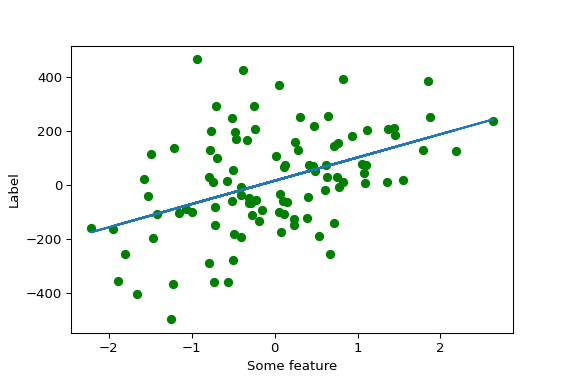
\includegraphics[width=0.7\linewidth]{../Implementation/Plots/linear_reg_example.png}
	\caption{}
	\label{fig:linearreg}
\end{figure}
One popular way of approximating hypotheses in linear regression is \textit{least squares}, which seeks to find coefficients $ w^{*}_j $, $ j = 1, \dots, p $ that minimize the squared differences across all N pairs the training set $ S $:
\begin{equation}
\argmin_{w} \sum_{i=1}^{N}(y_i - w_0 - \sum_{j=1}^{p} x_{ij}w_j)^2 
\end{equation}

\subsection{Tree-based ensembles}

As shown in the literature review, tree-based ensembles like GBDTs and Random Forests are popular in the field of arrival time estimation. Ensemble learning is motivated by the idea that so called \textit{base learners} (synonym to \textit{model} or \textit{hypothesis}) produce rather inaccurate results on their own, but form an accurate prediction model when they are combined. For tree-based ensembles, decision trees are used as base learners. 
Generally speaking, decision trees partition the feature space into distinct regions and then, in the case of regression, fit a real-valued prediction to each region. 
A single decision tree is given by
\begin{equation}
h(x) = \sum_{m=1}^{M} c_m I(x \in R_m)
\end{equation}
where $ c_m $ is the constant representing the prediction for all samples belonging to the m-th terminal region $ R_m $. Adopting the mean squared error as the loss metric, the predicted constant $ \hat{c}_m $ for each terminal region $ R_m $ is the average of all $ y $ for each $ x \in R_m $:
\begin{equation}
	\hat{c}_m =  \dfrac{1}{N_{R_m}}\sum_{x_i \in R_m}^{} y_i
\end{equation}
with $ N_{Rm} $ being the number of samples in terminal region $ R_m $. Given this, the decision tree algorithm needs to find optimal binary splits. Solving this analytically is computationally infeasible. Therefore, decision trees are constructed in a greedy fashion.
Let $ j $ be the split variable, representing the feature based on which the split of the feature space is done on, and $ s $ its associated split threshold.
The initial partition creates two disjoint regions
\begin{equation}
	R_1 (j,s) = \{X | X_j < s \}, R_{2} = \{X | X_j > s\}.
\end{equation}
The algorithm seeks optimal $ j $ and $ s $ by finding constants that minimize the overall loss, which in our case is measured with the mean squared error, for both terminal regions $ R_1 $ and $ R_2 $:
\begin{equation}\label{minjs}
	\min_{j,s} \bigg [\min_{\hat{c}_1} \sum_{x_i \in R_1(j,s)} \dfrac{1}{2}(y_i - \hat{c}_{2})^2 + \min_{\hat{c}_2} \sum_{x_i \in R_{2}(j,s)} \dfrac{1}{2}(y_i - \hat{c}_{2})^2\bigg]
\end{equation}
Having found the optimal split variable and split threshold, this procedure is repeated for each terminal region until a termination condition holds, e.g. a fixed maximal depth for the tree or a lower bound wrt. number of samples in each terminal region.
\newline
TODO: Disadvantages of decision trees (e.g. prone to overfitting, not as accurate as ensembles)
\newline
\newline
Knowing how CART builds regression trees, we now can advance to tree-based ensemble learning techniques which combine several regression trees to make predictions each in their own way.
The two ensemble learning approaches relevant for this work are \textbf{bagging}, , shorthand for \textit{bootstrap aggregating}, and \textbf{boosting}. 
Algorithms belonging to bagging first create bootstrap data sets $ S^{*} $ by randomly drawing samples with replacement from training data S, fit each $ S^{*b} $ a hypothesis $ h^{*b}(x) $ and take the average across all hypotheses as the bagging estimate: 
\begin{equation}\label{average}
	h_{bag}(x) = \dfrac{1}{B} \sum_{b=1}^{B} h^{*b}(x).
\end{equation}
Since decision trees are low in bias and high in variance due to their ability to capture complex mappings, averaging across all hypotheses reduces the variance because of the strong law of large numbers [<-- TODO: More detailed explanation].
Random Forests belong to the class of bagging algorithms and work as follows:
For an arbitrarily chosen and fixed amount of estimators $ B \in \mathbb{N}$, we create bootstrap data sets $ S^{*b} $ with $ b = 1, \dots, B $ of size $ N $ from the training data $ S $. The b-th regression tree $ T_b $ is grown to $ S^{*b} $ by first selecting a subset of $ m $ features with $ m \leq p $, and then growing a regression tree according to CART as described above.
Having grown each bootstrap data set $ S^{*b} $ its own regression tree $ T_b $, random forest for regression averages across all hypotheses of each regression tree by applying equation \ref{average} and returns
\begin{equation}
h^{B}_{rf}(x) = \dfrac{1}{B} \sum_{b=1}^{B} T_b(x)
\end{equation}
as the bagging estimate.
\newline
\newline
TODO: Introduce concept of boosting and GBDTs before diving deep into technical details.
\newline
\newline
The first step in GBDT is to initialize a model with a constant $ \hat{c} $ that minimizes the overall loss across all training samples.
\begin{equation}
h_{0}(x) =  \argmin_{\hat{c}} \sum_{i=1}^n L(y_i,\hat{c}) \label{gbdt_step1}
\end{equation}
Using mean squared error as the loss metric, the predictor minimizing the overall loss is simply the average of all $ y $.
Given the initial model $ h_0(x) $, M regression trees can now be build sequentially as shown in the following. 
The first step computes pseudo-residuals $ r_{im} $ between the prediction value of the former learner for the i-th sample $ h_{m-1}(x) $ and the actual i-th target for the m-th tree $ y_i $ by deriving the loss function w.r.t to $ h_{m-1}(x) $: 
\begin{equation}
	r_{im}\ = - \bigg[\dfrac{\delta L(y_i, h(x_i))}{\delta h(x_i)}\bigg]_{h(x) = h_{m-1}(x)}
\end{equation} 
for every i-th example.
In the second step, the algorithm fits a regression tree to every $ r_{im} $ and creates disjoint regions $ R_{jm} $ for $j = 1, ..., J_m$. 
In the third step, we compute: 
\begin{equation}
	\hat{c}_{jm} = \argmin_{\hat{c}} \sum_{x_i \in R_{ij}} L(y_i, h_{m-1}(x_i) + \hat{c})
\end{equation}
for every terminal region j in the m-th tree. 
Given this, we now update the former weak learner with the new one:
\begin{equation}
	h_m(x) = h_{m-1}(x) + \alpha \sum_{j=1}^{J_m} \hat{c}_{m}I(x \in R_{jm})
\end{equation}
where $ \alpha $ is the learning rate, and $ I(\cdot) $ is the indicator function. 


\subsection{Neural Networks for regression}


\begin{figure}[h]
	\centering
	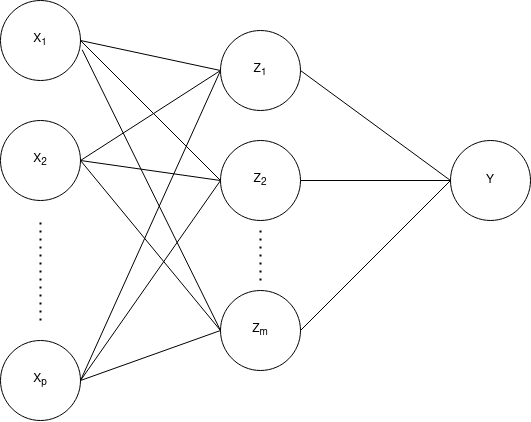
\includegraphics[width=0.5\linewidth]{../simplenn.png}
	\caption{Our neural network architecture to estimate arrival times: a single layer perceptron.}
	\label{fig:nnarchitecture}
\end{figure}


\section{Feature Selection}

As shown, researchers use different feature selection methods. A majority of the presented papers crafts features manually relying on domain expertise, whereas others (e.g \cite{Siripanpornchana2016_AnnWithDbnFS} and \cite{Huang2018_GBDT}) used representation learning techniques.
\newline
TODO: Manual feature selection
\newline 
TODO: Autoencoder
\newline
Maybe-TODO: Other feature selection methods, e.g. PCA?

\section{Hyperparameter Optimization}

\section{Evaluation} 
For accuracy: MSE 
\newline
Hyperparameter importance analysis for robustness
\newline
Noise einführen 
--> Wie reagiert Algorithmus auf Noise?
\newline
Anzahl der Trainingsdaten 
--> Wieviele Samples bis Konvergenz?
\newline
Feature Selection
--> Welches Features optimieren entsprechendes Modell bzgl. Runtime und Accuracy?

\chapter{Computational Study}

This chapter presents our computational study and is structured as follows: 
Section \ref{sec:data} describes the data our experiments are conducted on.
Section \ref{sec:samplesize} examines how different samples sizes used for training affect the test error.
In Section \ref{sec:hpo}, we optimize model hyperparameters and seek to get better intuition when for parameter configuration by analyzing parameters considered for our optimization.
Last but not least, section \ref{sec:noise} demonstrates how noise affects predictive performance of our models.

\section{Data exploration}\label{sec:data}
The available data set is provided by \cite{Hildebrandt2020_EAT} who created a high-dimensional data model with the RMDP instances originally used in \cite{UlmerRMDP}. It comprises 850.469 samples, 23.341 unique customer locations, a delivery fleet of 15 vehicles and 15 unique restaurant locations. The temporal and spatial distribution of the orders is depicted in figure \ref{fig:dists}. 
\begin{figure}[h]
	\centering
	\subfigure[Request arrival time distribution]{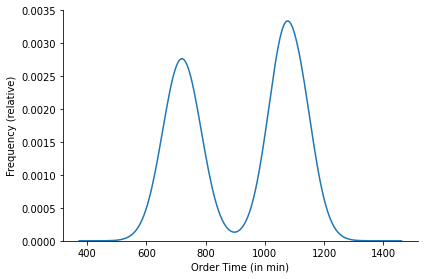
\includegraphics[width=0.49\linewidth]{../Implementation/DataDescription/order_time_dist.png}}
	\subfigure[Spatial distributions]{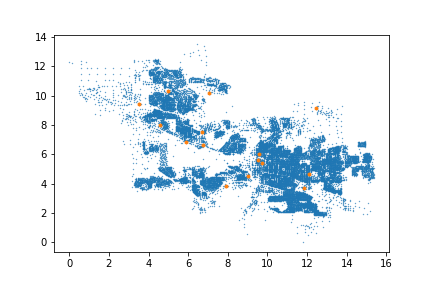
\includegraphics[width=0.49\linewidth]{../Implementation/DataDescription/spatial_dist.png}}
	\caption{Spatial and temporal distributions}
	\label{fig:dists}
\end{figure}

Panel (a) of figure \ref{fig:dists} shows the order behaviour of customers. The x-axis denotes the day time in minutes, the y-axis denotes the relative frequency of incoming customer orders for a given day time on the y-axis. We can observe that the order time behaviour across all customers follows a bimodal gaussian distribution. The order frequency peaks at around 12:00 a.m (roughly 700 minutes of day time) and again around 6.00 p.m (roughly 1100 minutes of day time). This indicates that the probability of an order taking place during lunch or dinner time is relatively high.  
Panel (b) of figure \ref{fig:dists} shows the spatial distribution of customer and restaurant locations. The x-axis depicts the  

\begin{figure}[h]
	\centering
	\subfigure[Delivery delay distribution]{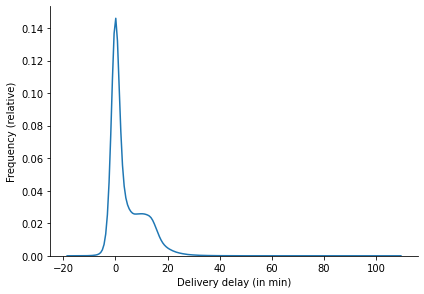
\includegraphics[width=0.49\linewidth]{../Implementation/DataDescription/delivery_delay.png}}
	\subfigure[Meal preparation time distribution]{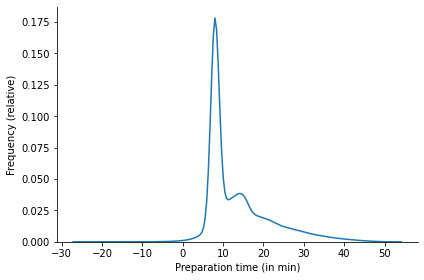
\includegraphics[width=0.49\linewidth]{../Implementation/DataDescription/prep_time.png}}
	\caption{Spatial and temporal distributions}
	\label{fig:prepdelay}
\end{figure}
Panel (a) of figure \ref{fig:prepdelay} shows the distribution of delivery delay times in minutes for all requests in the data. The delivery dela is here defined as the difference between actual and the expected time of arrival based on PoM. First, we observe that roughly 14-15\% of the requests in our data are delivered on time. Negative values for the delivery delay on the plot indicate that a rather tiny amount of orders happens to be delivered earlier than expected. However, we are most interested in the orders that are actually delivered later than expected. We observe that a non-trivial amount of orders is delivered with a delay of up to 20 minutes. As we will later show, arrival time estimation via supervised learning is a vastly better option compared to planning on means.
Since arrival times are impacted by uncertainty in meal preparation times, we take a look at their distribution in our data as well. In panel (b) of figure \ref{fig:prepdelay}, we observe that roughly a fifth of the orders had a preparation time of around 10 minutes. However, a non-trivial amount of orders seem to have quite longer preparation times ranging from 15 to less than 40 minutes. 

\section{Experiment: Sufficient Sample Sizes}\label{sec:samplesize}

This section compares how a difference sample size impact the test error for each possible combination of models and datasets. With this experiment, we intend to examine how different sizes in training data affect the test error for the respective combination. Since less samples in the training data corresponds to lower training times, we use the results of this experiment for the subsequent hyperparameter optimization and the noise analysis to speed our experimental procedure up. For our linear model and the considered ensembles, we consider 100 training runs with every run corresponding to a sample subset size $ \{2000, 4000, \dots, 200.000\} $. For each model, we set the parameters manually since we did not conduct hyperparameter optimization yet. 

\begin{figure}[h]
	\centering
	\subfigure[For GBDT]{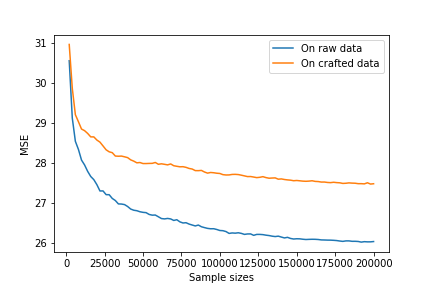
\includegraphics[width=0.49\linewidth]{../Implementation/SampleSize/GBDT_SampleSizes.png}}
	\subfigure[For Random Forest]{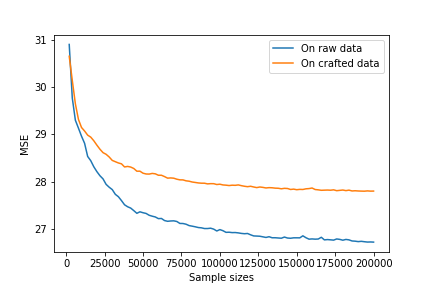
\includegraphics[width=0.49\linewidth]{../Implementation/SampleSize/RF_SampleSizes.png}}
	\subfigure[For Linear Regression]{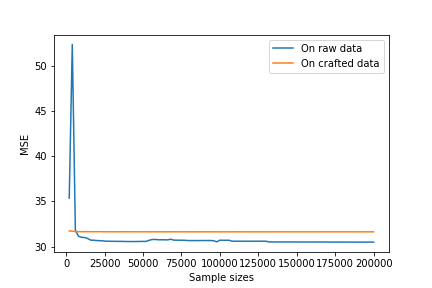
\includegraphics[width=0.49\linewidth]{../Implementation/SampleSize/LR_SampleSizes.png}}
	\caption{MSE for different sample sizes}
	\label{fig:convergences}
\end{figure}

[TODO: Explain results]
\section{Experiment: Hyperparameter Optimization}\label{sec:hpo}
This section presents the hyperparameter optimization (HPO) experiments conducted for GBDT and Random Forest.
We use \textit{Optuna}, a popular HPO framework proposed and designed by \cite{akiba2019optuna}, to conduct our HPO experiments. 
\textit{Optuna} provides a simple implementation design that allows us to analyze several parameters of choice from different points of view. 
The optimizations were conducted on both the crafted data set and the raw data set. 
Concretely, we will proceed as follows: First, we will present the hyperparameters we decided to include in the HPO to then in turn present the optimal hyperparameter values resulting from the experiment and explore the predictive power of different parametrizations. 
For every GBDT and RF experiment instance, the hyperparameters will be sampled via the \textbf{C}ovariance \textbf{M}atrix \textbf{A}daption \textbf{E}volution \textbf{S}trategy, or in short \textbf{CMA-ES}. 
\textit{CMA-ES} follows a simple principle: The probability of samples from previously succesful optimization steps being drawn again is positively correlated to the contribution of those samples to the objective. For further information on \textit{CMA-ES}, the reader is referred to \cite{hansen2016cma}. 
To speed up the optimization process, we use the \textit{Optuna}-implementation of the \textit{Hyperband Pruner} presented in \cite{li2018hyperband} and furthermore use only 200.000 of our samples since the models begin to converge at this subset size as shown in section \ref{sec:samplesize}. By that, we hope to get a fine-tuned model that maximizes prediction quality on one hand, and intuition for suitable parametrizations on the other hand.
In the next step, we will use the \textit{optuna} implementation of the \textit{fANOVA} evaluation algorithm presented in \cite{fANOVA} to determine hyperparameter importances. 
In short, \textit{fANOVA} calculates feature importances by fitting a random forest regression model to the optimal parameter configuration that results of the HPO with which it aims to predict the corresponding objective value. The relative importances provide information about the parameter variances. A higher value is associated with a higher variance, meaning that a change of the parameter setting will have a greater impact on the prediction performance compared to parameters of low relative importance. Thereby, we can assess which parameters impact the model significantly and which parameters are less significant, and especially how the importances differ for the two data sets. For each parameter importance prediction, we set the number of estimators in \textit{fANOVA} to 1000.
\subsection{GBDT}

In this subsection, we will conduct HPO experiments for GBDTs on both datasets. 
For GBDT, we decided to optimize following parameters and set the search spaces for each of them as follows:
\begin{description}[font=$\bullet$\scshape\bfseries]
	\item $ \text{learning\_rate} \in [0.01, 0.05] $  in steps of 0.001.
	\item $ \text{max\_depth} \in [5, 100] $ in steps of 0.001.
	\item $ \text{feature\_fraction} \in [0.1, 1.0] $ in steps of 0.01.
	\item $ \text{feature\_fraction\_bynode} \in [0.3, 1.0] $ in steps of 0.01
	\item $ \text{num\_leaves} \in [20, 300] $ in steps of 1
	\item $ \text{min\_child\_samples} \in [10, 400] $ in steps of 1.
	\item $ \text{subsample\_freq} \in [1, 10] $ in steps of 1.
	\item $ \text{subsample} \in [0.3, 1.0] $ in steps of 0.01.
\end{description}
Besides the parameters considered for optimization, we set the number of estimators for one iteration in GBDT to 1000 and enable early stopping with a patience of 20. Our selection of parameter search spaces is the result of trial-and-error since machine learning problems are highly individual and, as we have already demonstrated with our literature review, different solution approaches for quite similar problems are possible. The determination of parameter values and parameter search spaces therefore has to happen at least partly in a manual fashion, which is why we regard the trial-and-error heuristic as a suitable approach for the configuration of hyperparameter values and hyperparameter search spaces for our HPO. Detailed descriptions of the considered parameters for the \textit{lightgbm}-GBDT implementation can be found under \url{https://lightgbm.readthedocs.io/en/latest/Parameters.html}.

The exact optimal parameter configuration for GBDT on both data sets is depicted in figure \ref{fig:GBDT_Optimal}. Training GBDT with the optimal parameter configuration using the full available amount of samples results in a mean squared test error of approximately 25.1384 on the raw data, and 27.0852 on the crafted data. Early Stopping does not set in when training GBDT on raw data, whereas it does set in for the crafted data at around 600. 
\begin{figure}[h]
	\centering
	\subfigure[Optimal configurations]{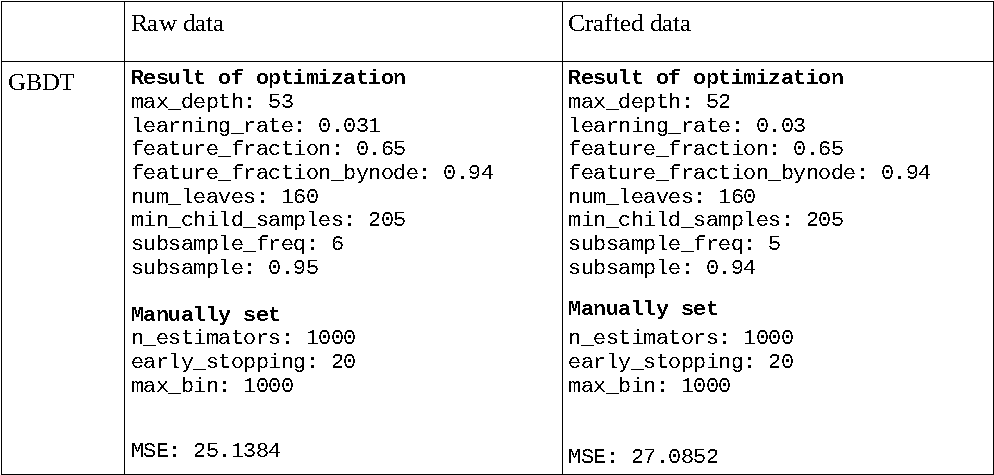
\includegraphics[width=\linewidth]{figures/HPO/GBDT_ResultsTable_HPO_Optimal.pdf}}
	\subfigure[Training history on crafted data]{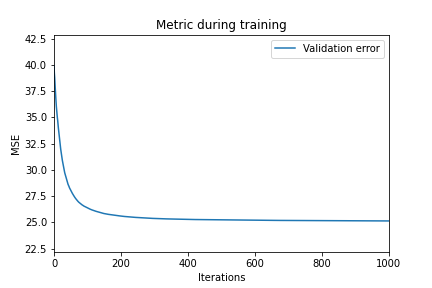
\includegraphics[width=0.49\linewidth]{../Implementation/optunaStudies/GBDT_Raw_Optim_Metric.png}}
	\subfigure[Training history on crafted data]{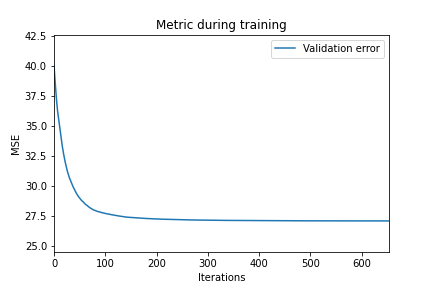
\includegraphics[width=0.49\linewidth]{../Implementation/optunaStudies/GBDT_Crafted_Optim_Metric.png}}
	\caption{Optimal configurations and training histories for GBDT}
	\label{fig:GBDT_Optimal}
\end{figure}

Figure \ref{fig:GBDT_ParallelPlot} depicts the parameter configurations of each optimization epoch in form of a parallel coordinate plot for GBDT on raw data in panel (a) and on crafted data in panel (b). Except the vertical gray line one the very left in the plots, each vertical gray axis represents the values ranging within the defined intervall of its corresponding parameter, whereas the very left line represents the axis for the objective values. The lines connecting all the parameter axes represent the parameter configurations of the optimization epochs. The bluer a line, the better the objective value - in our case the mean squared error. 
At first glance, it can be seen directly that the parameter configurations of both plots for good predictive performance are quite similar. For both sets, the mean squared error is minimized when we roughly use two-thirds of the features for each GBDT iteration (feature\_fraction, feature\_fraction\_bynode). Less test error is more likely achieved when we allow the algorithm to build rather deep trees up to a maximal depth of 50 while constraining the tree splitting process by specifying a lower bound of around 200 for the minimal amount of samples a node must contain in order to split it further (min\_child\_samples). We can furthermore see that a better objective value is attained when using nearly all samples considered for a GBDT iteration rather than applying (subsampling) and learning rates ranging between 0.03 to 0.05 (learning\_rate).

\begin{figure}[h]
	\centering
	\subfigure[On raw data]{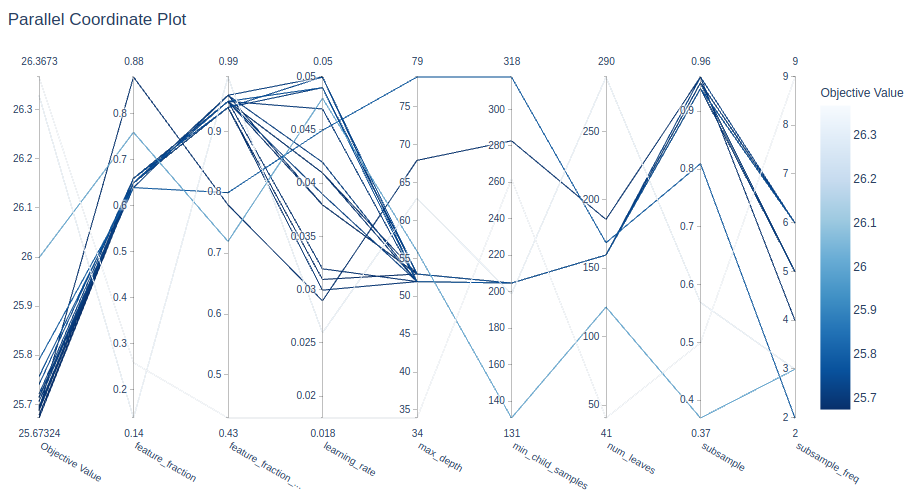
\includegraphics[width=\linewidth]{figures/HPO/GBDT_HPO_Raw_ParallelPlot.png}}
	\subfigure[On crafted data]{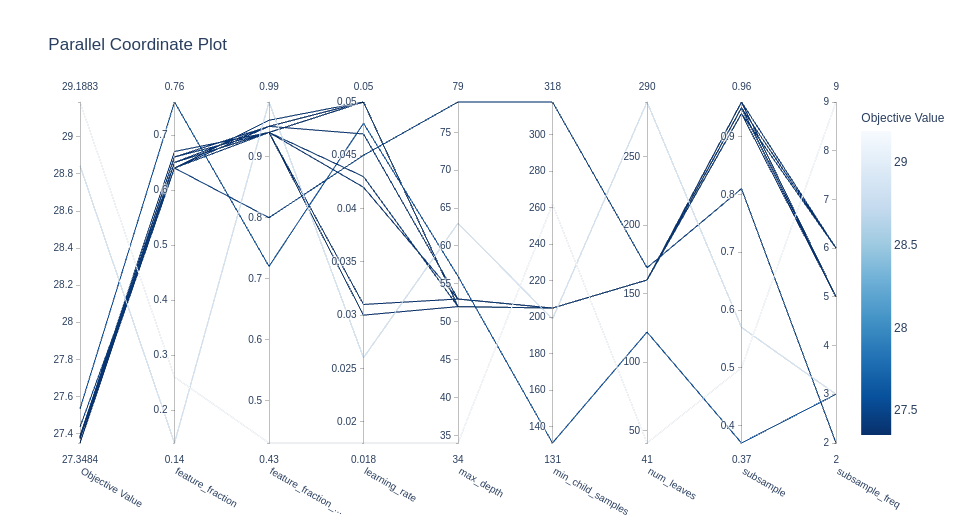
\includegraphics[width=\linewidth]{figures/HPO/GBDT_HPO_Crafted_ParallelPlot.png}}
	\caption{Parallel Coordinate Plots for GBDT}
	\label{fig:GBDT_ParallelPlot}
\end{figure}

Up next are the hyperparameter importances of GBDT depicted in figure \ref{fig:GBDT_Importances}. Panel (a) shows the importances for GBDT when trained on raw data
Panel (b) shows the importances for GBDT when trained on crafted data.
The x-axis of the importance plots depicts the relative parameter importances. 
On the y-axis is categorical and shows the parameters we considered to optimize. 
We can observe that the results for the datasets GBDT was trained on differ significantly. 
For GBDT on the raw data, we observe that choosing the right amount for subsampling, a suitable learning rate for calculating the gradient in GBDT, and the right feature fraction are of highest importance. For GBDT on the crafted data, we observe that the learning rate and the feature fractio are of even more relative importance, whereas the parameter for subsampling has far less significant impact on the objective value as compared to GBDT on raw data. 
We observe further non-trivial differences (here: $ \geq 5\%$ ) in relative importance for the subsampling frequency showing a difference 7\%, and for \textit{min\_child\_samples} with a difference of 5\%. For both datasets, the number of leaves, the percentage of features fractioned per node, and the maximal depth constraint for the estimators remain nearly equally important.   
\begin{figure}[h]
	\centering
	\subfigure[On raw data]{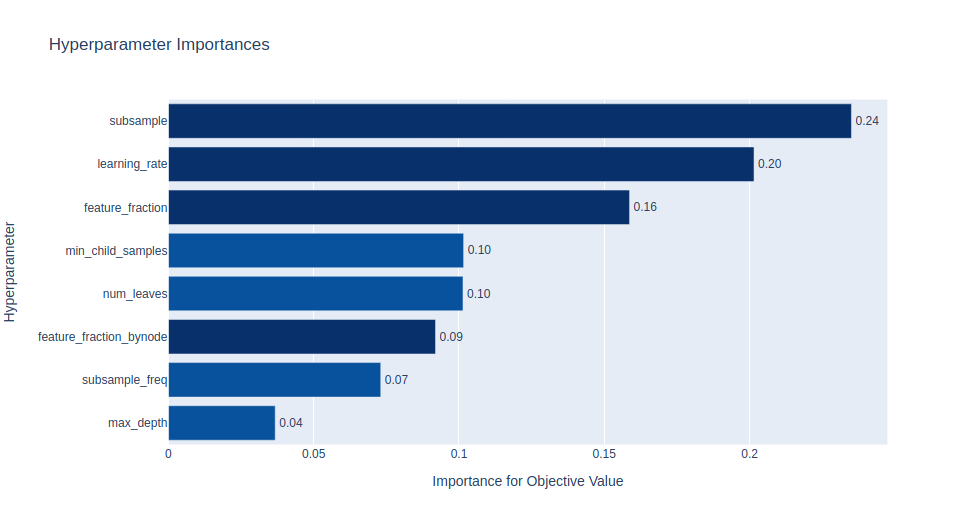
\includegraphics[width=\linewidth]{figures/HPO/GBDT_HPO_Raw_Importances.png}}
	\subfigure[On crafted data]{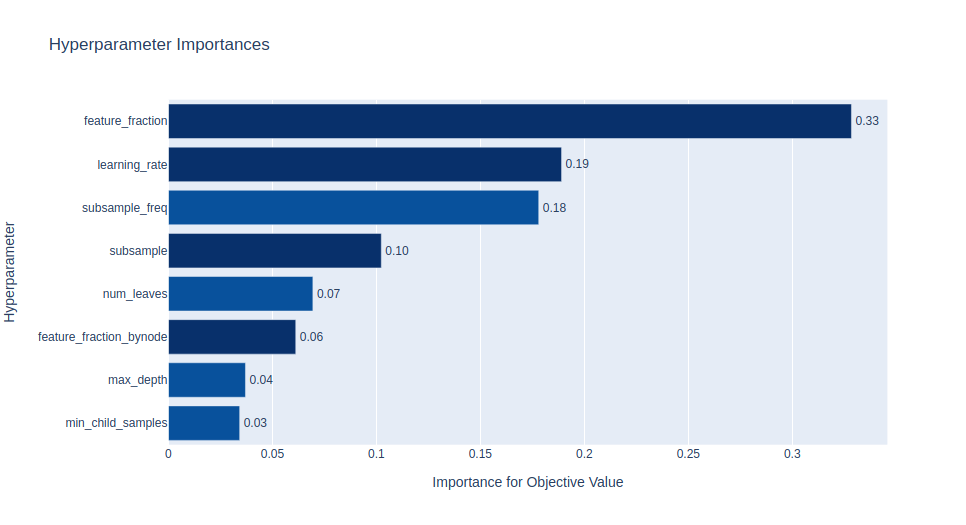
\includegraphics[width=\linewidth]{figures/HPO/GBDT_HPO_Crafted_Importances.png}}
	\caption{Hyperparameter Importances for GBDT}
	\label{fig:GBDT_Importances}
\end{figure}

Although there are significant differences between the hyperparameter importances for both GBDT experiment instances, the resulting optimal configuration of both does hardly differ as we have already pointed out. Thereby, we suggest that the difference in relative parameter importances does not affect the outcome of the optimization. We also suggest that the importances depend on the features that are used. We further found that the raw set achieves significant less test error than the crafted data set. This could be due to the reason that, besides the maximal time shift features, our raw set includes exactly any routing information of a customer's route that the state space of the RMDPEAT contains, whereas the crafted set includes only the amount of total stops, pick-up stops, and delivery stops. 
\clearpage
\subsection{Random Forest}
In this subsection, we will conduct HPO experiments for Random Forest on both datasets. 
For Random Forest, we decided to optimize following parameters and set the search spaces for each of them as follows:
\begin{description}[font=$\bullet$\scshape\bfseries]
	\item $ \text{max\_depth} \in [5, 100] $ in steps of 1.
	\item $ \text{feature\_fraction} \in [0.3, 1.0] $ in steps of 0.01.
	\item $ \text{feature\_fraction\_bynode} \in [0.3, 1.0] $ in steps of 0.01
	\item $ \text{num\_leaves} \in [900, 1200] $ in steps of 1
	\item $ \text{subsample\_freq} \in [1, 10] $ in steps of 1.
	\item $ \text{subsample} \in [0.3, 0.99] $ in steps of 0.01.
\end{description}
Besides the parameters considered for optimization, we set the number of estimators for one iteration in Random Forest to 1000 and enable early stopping with a patience of 20 as we did for the GBDT optimization. Additionally, we set \textit{min\_child\_samples} to 1 and thus exclude it from the set of parameters considered for optimization, because we found by trial-and-error that \textit{lightgbm-RF} performs best when it is set very low. We further set the parameter \textit{min\_data\_in\_bin} to 1 as we have again found by trial-and-error that this works well for \textit{lightgbm-RF}. Again, We are going to analyze optimal configurations with the help of the corresponding parallel plots first and then examine the hyperparameter importances for Random Forest for each dataset. 

Figure \ref{fig:RF_Optimal} depicts the optimal parameter configurations resulting of the HPO for the considered parameters and the respective training histories. Again, we observe that Random Forest on the raw data returns a lower test error of 26.5538 compared to the crafted features with a mean squared error of 27.7938 when trained on their respective optimal parameter configurations. Early Stopping sets in at around 170 iterations for the raw data instance, and at roughly 70 for the crafted data experiment instance. 
\begin{figure}[h]
	\centering
	\subfigure[Optimal configurations]{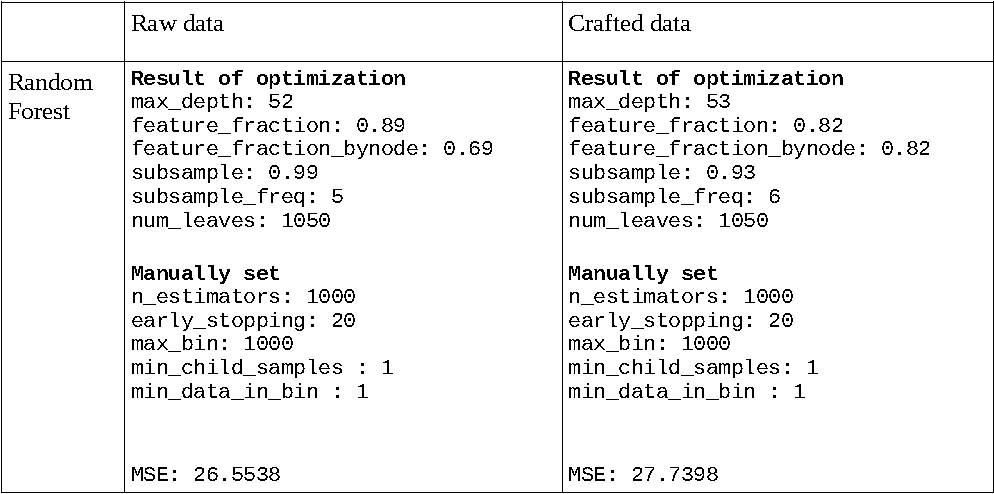
\includegraphics[width=\linewidth]{figures/HPO/RF_ResultsTable_HPO_Optimal.pdf}}
	\subfigure[Training history on raw data]{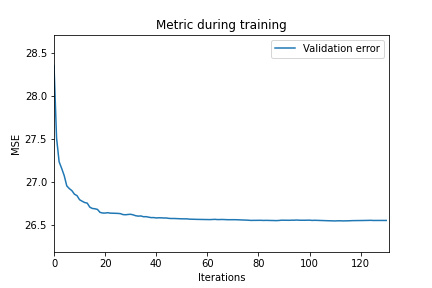
\includegraphics[width=0.49\linewidth]{../Implementation/optunaStudies/RF_Raw_Optim_Metric.png}}
	\subfigure[Training history on crafted data]{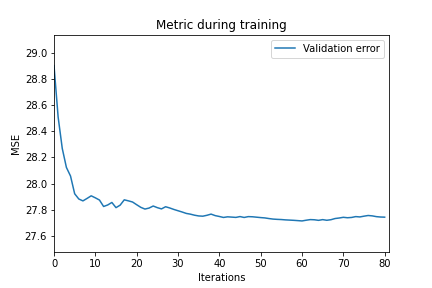
\includegraphics[width=0.49\linewidth]{../Implementation/optunaStudies/RF_Crafted_Optim_Metric.png}}
	\caption{Optimal configurations and training histories for Random Forest}
	\label{fig:RF_Optimal}
\end{figure}
Figure \ref{fig:RF_ParallelPlot} depicts the parallel coordinate plots for Random Forest on the raw and crafted features in panel (a) and (b) respectively. We observe that the distribution of parameter configurations achieving a comparably well objective value, is quite similar. A minimized objective value is achieved when the feature fraction and the feature fraction by node used for each estimator range between 0.8 and 1. Further, the maximal depth constraint set at a rather high value ranging between 50 and 60 seems to be optimal according to the HPO. The number of leaves each estimator has at the end of the iteration lies at roughly 1050 in most optimal cases. For subsampling, we observe that subsampling fraction greater than 90\% in a frequency of 6 goes is correlated to a minimized test error.
\begin{figure}[h]
	\centering
	\subfigure[On raw data]{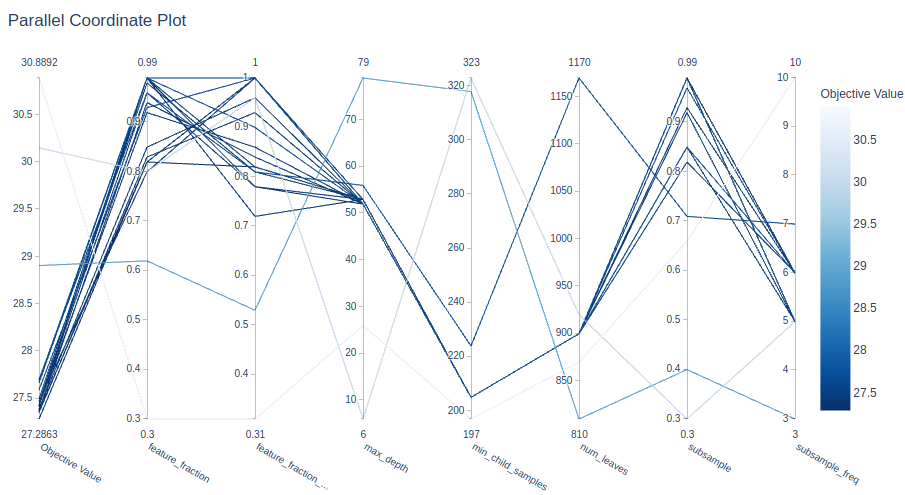
\includegraphics[width=\linewidth]{figures/HPO/RF_HPO_Raw_ParallelPlot.png}}
	\subfigure[On crafted data]{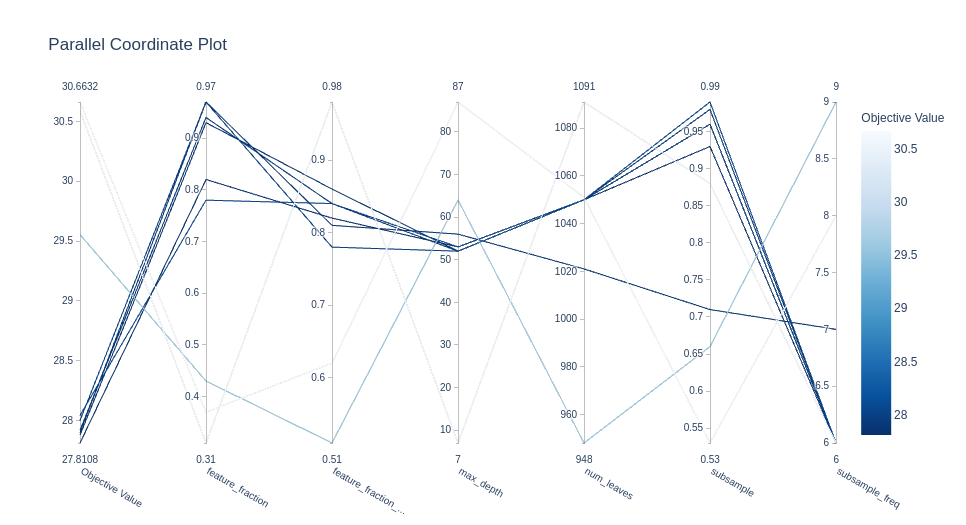
\includegraphics[width=\linewidth]{figures/HPO/RF_HPO_Crafted_ParallelPlot.png}}
	\caption{Parallel Coordinate Plots for Random Forest}
	\label{fig:RF_ParallelPlot}
\end{figure}

The hyperparameter importances for Random Forest on the raw and the crafted data are depicted in \ref{fig:RF_Importances}. For both instances, we observe that the chosen feature fraction has by far the most impact with a relative importance of 0.43 for the raw data instance, and 0.48 for the crafted data instance. Combining this information with the information given on the parallel plot, we conclude that it is crucial to set the feature fractions higher than 80\%. The instances significantly differ when it comes to subsampling and the subsampling frequence with differences of 10\% and 11\% respectively. When it comes to the maximum permitted depth and the number of leaves, the instances also show a percentual difference of 6\% and 3\% respectively.
\begin{figure}[h]
	\centering
	\subfigure[On raw data]{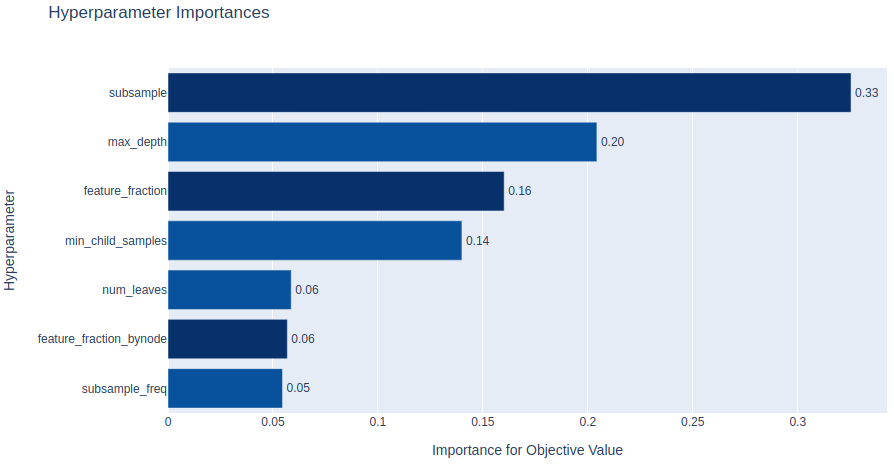
\includegraphics[width=\linewidth]{figures/HPO/RF_HPO_Raw_Importances.png}}
	\subfigure[On crafted data]{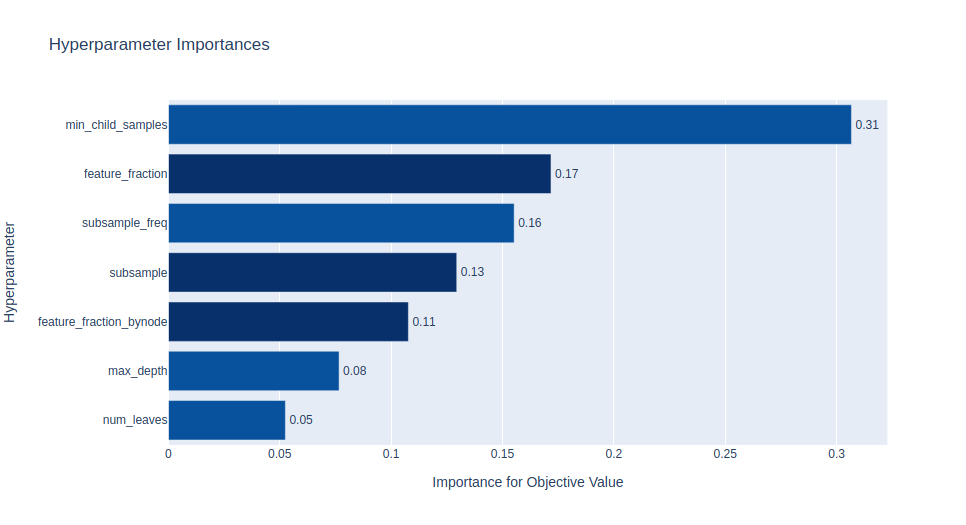
\includegraphics[width=\linewidth]{figures/HPO/RF_HPO_Crafted_Importances.png}}
	\caption{Hyperparameter Importances for Random Forest}
	\label{fig:RF_Importances}
\end{figure} 
 
\section{Experiment: Adding Noise}\label{sec:noise}
In this experiment, we test the robustness of our models on full sample size. We do this by randomly sampling values from the gaussian distribution
\begin{equation}
	p(x) = \dfrac{1}{\sqrt{2\pi\sigma^{2}}} e^{-\dfrac{(x-\mu)^2}{2\sigma^2}}
\end{equation}
with a mean $ \mu $ of 1 and standard deviations $ \sigma \in \Sigma $ in the set of $ \{0.1, 0.2, \dots, 1.0\} $ and adding the resulting value, which is the noise, to the order time, the meal preparation time and the PoM-based expected time of arrival. A higher standard deviation is understood as a wider spread of the distribution, and vice versa. The GBDTs and Random Forests were trained on with the optimal parameter configurations resulting from the HPO. Figure \ref{fig:noise} depicts the model performances for different levels of noise on both datasets. The x-axis represents the standard deviation, the y-axis shows the mean squared test error. As opposed to the GBDT and Random Forest, we  At first glance, we observe that a higher test error is associated with higher levels of noise for every test instance. GBDT and Random Forest trained on the raw data produce the best results. For them, we observe quite similar behaviour when trained on the different datasets: While both start out fairly close to the value attained in figure \ref{fig:GBDT_Optimal} and \ref{fig:RF_Optimal} with a mean squared error of approximately less than 26 and 28 respectively on the raw set, both show a monotonous increase in test error up to approximately 30 for the highest noise level considered. However, we get significantly different results when we train GBDT and Random Forest on the crafted set. For both models, the MSE starts out with a mean squared error around 30, which is noticeably less than the mean squared error achieved with the configurations for the crafted set depicted in \ref{fig:GBDT_Optimal} and \ref{fig:RF_Optimal}, and rise up to slightly more than 36. We thus conclude that the models trained upon the raw set are significantly more robust when noise is induced. Our linear model produced results that are highly interesting: Despite both (c) and (d) visualizing quite similar looking exponential increases, the resulting MSEs for the different noise levels could not be further away from each other. When trained on raw data, linear regression levels off between 30-31 and is therefore the most robust model in our comparison since its variability in results is by far the lowest. When trained on crafted data however, a consideration of linear regression as a prediction model is no longer an option as the MSE skyrockets to 1200 at a noise level of 1.0. We further note that linear regression on the raw data consistently produces better results than GBDT and Random Forest when trained on the crafted data. 
Wrt. to the robustness of our models, we conclude the following:
\begin{description}[font=$\bullet$\scshape\bfseries]
	\item Whether we use the raw or the crafted data set for training, GBDT and Random Forest produces the best results. On raw data, GBDT is ahead of random forest, whereas both perform nearly equally good when trained on the crafted data set. 
	\item Linear Regression is robust to noise the most on the raw data. Surprisingly, the complete opposite is true when we train linear regression on the crafted data. 
\end{description}
\begin{figure}[h]
	\centering
	\subfigure[For GBDT]{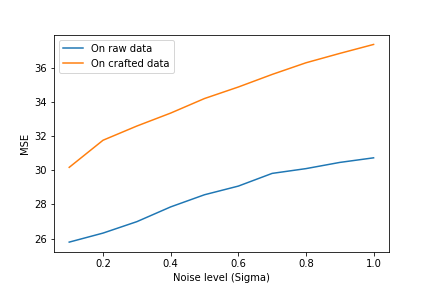
\includegraphics[width=0.49\linewidth]{../Implementation/NoiseStudies/GBDT_Noise.png}}
	\subfigure[For Random Forest]{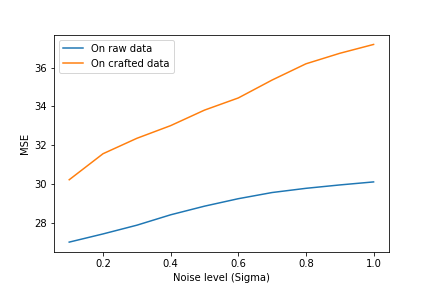
\includegraphics[width=0.49\linewidth]{../Implementation/NoiseStudies/RF_Noise.png}}
	\subfigure[For Linear Regression (Raw)]{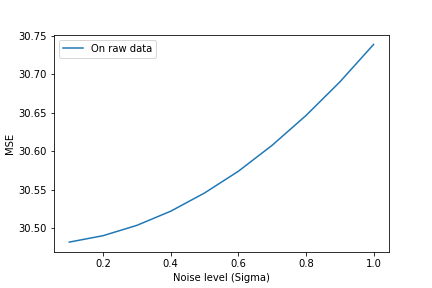
\includegraphics[width=0.49\linewidth]{../Implementation/NoiseStudies/LR_Raw_Noise.png}}
	\subfigure[For Linear Regression (Crafted)]{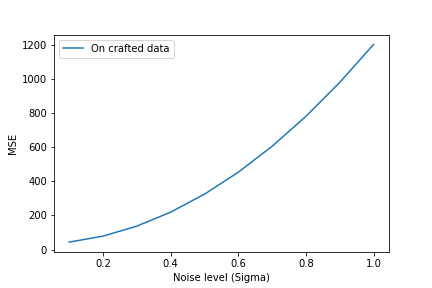
\includegraphics[width=0.49\linewidth]{../Implementation/NoiseStudies/LR_Crafted_Noise.png}}
	\caption{Performance of models for different noise levels on both datasets}
	\label{fig:noise}
\end{figure}




\chapter{Conclusion}



%%% ------------- Ende Textteil -------------

%%% Anhang
\bibliography{references}%%% obligatorisch         
%\anhang                 %%% optional, in der Datei anhang.tex

\end{document}
